\documentclass[12pt,twoside]{article}

\usepackage{amsmath}
\usepackage{fancyhdr}
\usepackage{graphicx}
\usepackage{amssymb}
\usepackage{wrapfig} %wrap images in text
%\usepackage[UTF8]{ctex} %display chinese
\usepackage[colorlinks=true, linkcolor=red, urlcolor=blue, citecolor=blue]{hyperref}

\newenvironment{tight_enumerate}{
\begin{enumerate}
  \setlength{\itemsep}{0pt}
  \setlength{\parskip}{0pt}
}{\end{enumerate}}

\newenvironment{tight_itemize}{
\begin{itemize}
  \setlength{\itemsep}{0pt}
  \setlength{\parskip}{0pt}
}{\end{itemize}}

\setlength{\oddsidemargin}{0pt}
\setlength{\evensidemargin}{0pt}
\setlength{\textwidth}{6.5in}
\setlength{\topmargin}{0in}
\setlength{\textheight}{8.5in}
\setlength{\headheight}{15pt}

\newcommand{\andrew}{Andrew Xia}
\newcommand{\name}{6.115 Final Project Lab Notebook}
\renewcommand{\thesubsection}{\thesection.\alph{subsection}}
\renewcommand{\sectionmark}[1]{\markboth{#1}{}} % set the \leftmark


\pagestyle{fancy}
\fancyhead[R]{\andrew}
\fancyhead[L]{\leftmark} % 1. sectionname
\fancyhead[C]{\name}


\begin{document} 
\begin{center} {\bf \Large \name}
\\ \emph{3D Tic Tac Toe}
\\ {\bf \andrew}
\end{center}
\section{Overview}
{\em April 20, 2016 Proposal:} For my final project, I hope to build a 3D touchless tracking interface and connect it with my 8051 and PSoC to allow users to play 3D tic tac toe with either each other or a computer AI. 
\\
\\ \emph{What interested you in the idea?} I am interested in this idea because I want to work on a project that has both an interesting and flashy hardware and software component. Writing the AI software for my 3D tic tac toe board will be a very rewarding and educational experience for me, and building the 3D tracing interface will also be very fun. 
\\ 
\\ \emph{Why is this project interesting?} This project is interesting because while 2D tic tac toe is a game familiar to all, 3D tic tac toe represents a game that while it is familiar, it can also be novel and entertaining. This project also uses a 3D touchless interface for user input, which is another novel way of interacting with software, as we are used to touching buttons or screens to communicate with devices in our daily lives. 

\subsection{Hardware Overview}
The key hardware component of my project will be building a 3D touchless interface, which is shown in the image to the side. The three aluminum foils (or a similar material) on the three sides are the capacitors that the human finger complements, and thie distance from each of the three capacitors will definite the capacitance of the capacitance, which we can measure using an ADC, and effectively pinpoint the 3D location of the human hand. 
\\ I will use a 74LS245 chip to connect my PSoC to a VGA cable which can then display information on a screen. I will use what was covered in lecture to complete this task. 
\\ Below is a preliminary hardware schematic of my final project:
\begin{center}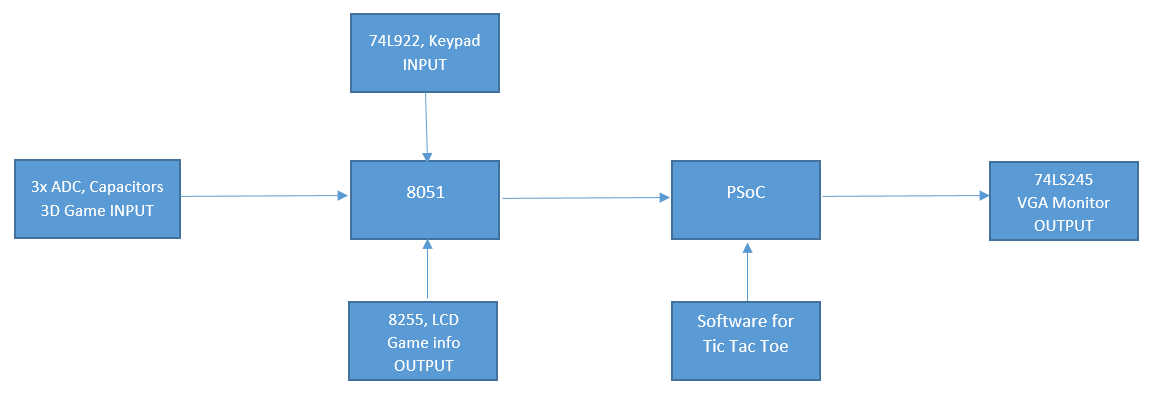
\includegraphics[width = 120mm]{../Proposals/Hardware_final.png} \end{center}

\subsection{Software Overview}
As for my software, I will code my project in C, using the PSoC as my main control module, as it would would be more efficient to do so over writing code in assembly for the 8051. The Tic Tac Toe AI is not too software heavy, so I hope to develop the basic framework for my code and spend the rest of my extra time focusing on hardware improvements. 
\\ Here is the high level software workflow for my final project:
\begin{center}\fbox{\begin{minipage}{35em}

\begin{tight_enumerate}
\item Initiate \& Reset Tic Tac Toe Board
\item Mode 1: two player Tic Tac Toe
	\begin{tight_enumerate}
	\item User can view \& rotate, using 74L922 or capacitive-based sensors, current 3D tic tac toe board on VGA display
	\item User adds piece to the board by leaving hand in position of 3D touchless tracking interface for extended amound of time
	\item After entering piece on board, the other player can play. 
	\end{tight_enumerate}
\item Mode 2: one player AI Tic Tac Toe
	\begin{tight_enumerate}
	\item User can view \& rotate, using 74L922 or capacitive-based sensors, current 3D tic tac toe board on VGA display
	\item User adds piece to the board by leaving hand in position of 3D touchless tracking interface for extended amound of time
	\item After entering piece on board, computer plays against user and submits his move through AI algorithm. 
	\end{tight_enumerate}
\item Reset the game and enter either mode through the 74C922 Keypad
\end{tight_enumerate}

\end{minipage}} \end{center}

\subsection{Format of my Lab Notebook}
I plan on formatting my lab notebook in this latex file, in which each day I work on the lab will be a section, and I can also reorganize my lab notebook to be thematically organized by the module that I will work on. 
\\ Each day, or section, will contain an {\em introduction} section in which I discuss the goals that I have for the day, and I will detail the tasks that I will work on in the subsections for each day. 

%%%%%%%%%%%%%%%%%%%%%%%%%%%%%%%%%%%%%%%%%%

\newpage
\section{April 21, 2016}
Goals I have for today / {\bf done} if task completed
\begin{tight_itemize}
\item Set up github for version control of my lab notebook and code {\bf done}
\item Build my initial capacitance based sensor
\item Set up my computer so I can code in C {\bf done}
\end{tight_itemize}

\subsection{Setting up github}
I am following the tutorial \href{https://help.github.com/articles/adding-an-existing-project-to-github-using-the-command-line/}{here} to create a new github repository. It will be located in my 6.115 dropbox folder, and on my github account under the repository \href{https://github.com/qandrew/6.115-final-project}{6.115-final-project}

\subsection{Building my initial capacitance based sensor}
References include this \href{http://makezine.com/projects/a-touchless-3d-tracking-interface/}{Makezine link}. 
\\ Notes on building a capacitance based sensor:
\begin{tight_enumerate}%[itemsep=5mm]
\item Beacuse humans have very little capacitance $~ 10 pF$, the time constant to which the plate would charge up based on the distance of the finger to the plate should be very small. Thus, I may need to think of more intelligent methods to build an effective capacitance based sensor. 
\item I can design different circuits
\end{tight_enumerate}

\subsection{Software development}
To install {\bf C}, I am following this \href{https://en.wikibooks.org/wiki/C_Programming/What_you_need_before_you_can_learn}{website} to install a C compiler for my computer. It is in fact better to code in Linux rather than $C$, so I will be using linux/ubuntu when needing to test my Tic Tac Toe code on my computer.
\\
\\ To install the Cypress PSoC creator IDE, I am following the instructions \href{http://www.cypress.com/products/psoc-software}{here}. Having PSoC Creator on my computer should help increase my productivity and workflow. 
\\
\\ I completed a two player Tic Tac Toe game coded using python today. The logic of the game is documented in my code. I plan on investigating more into AI algorithms, potentially using minimax or alpha beta pruning. \href{http://www.half-real.net/tictactoe/}{This website} has pretty good information on evaluation methods and algorithms for 3D Tic Tac Toe. 
\begin{center}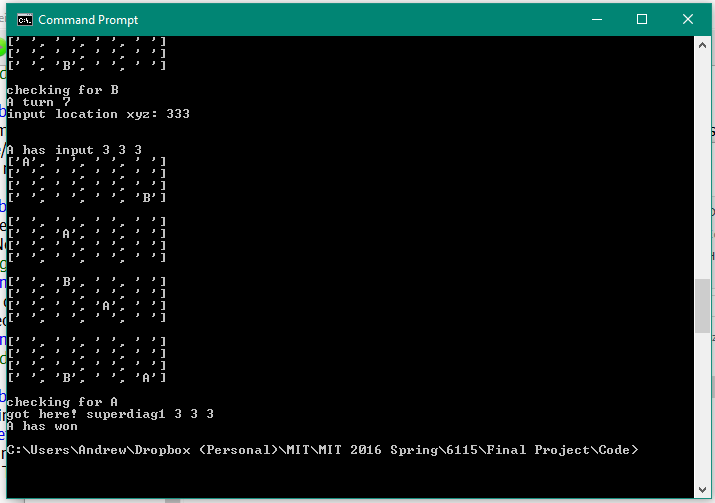
\includegraphics[width = 100mm]{Pics/4-21python.png} \end{center}
Above is an image of my python 3D tic tac toe script running

%%%%%%%%%%%%%%%%%%%%%%%%%%%%%%%%%%%%%%%%%%

\section{April 24 2016}

Goals I have for today / {\bf done} if task completed
\begin{tight_itemize}
\item Learn how to use Cypress EDS Laser Cutter  {\bf done}
\item Look into VGA connection to PSoC, how to connect my capacitance based sensor
\end{tight_itemize}
\begin{wrapfigure}{R}{0.3\textwidth}
\centering

\includegraphics[width = 30mm]{Pics/4-24b.jpg} 
\caption{\label{fig:frog1}test.} 
\end{wrapfigure}
\subsection{Using the Cypress EDS Laser Cutter}
I printed out a circular acryllic piece today with ny name on it. Some things to remember: I should use CorelDRAW or solid works to design my cuts. The {\em red} line must be set to hairline width for cuts. The {\em blue} line must be set to hairline width for scones. The {\em black} areas must can be set to anything for rasters. 

\subsection{Working on my capacitance based sensor}
The initial circuit that I tested did not work. It was picking up a lot of 60Hz noise (which is coming from the AC power that exists all around the lab). The top resistor has value $220k\Omega$ and the bottom resistor has value $10k\Omega$. 
%\begin{wrapfigure}{R}{0.3\textwidth}
%\centering
\begin{center} 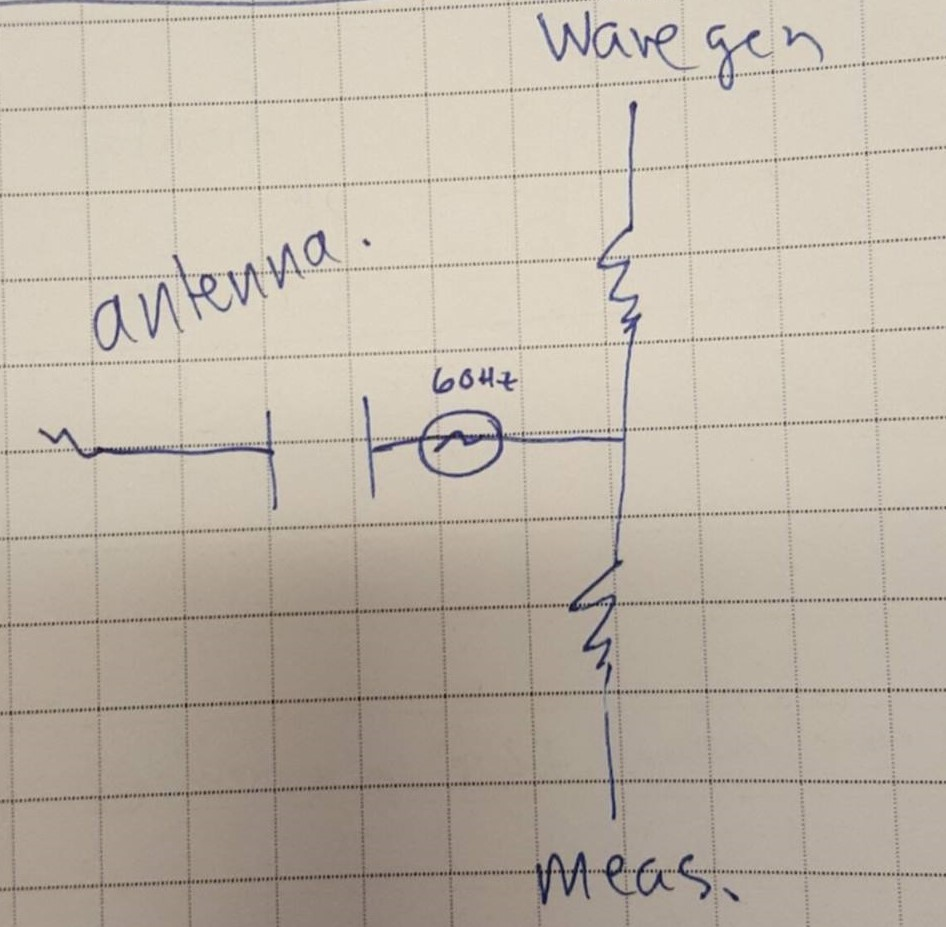
\includegraphics[width = 50mm]{Pics/4-24a.jpg}  \end{center} %\caption{\label{fig:frog1}test.} 
%\end{wrapfigure}
This circuit does not work.
\\ 
\\ I am now trying a new circuit, designed as follows according to the Makezine article
\begin{center} 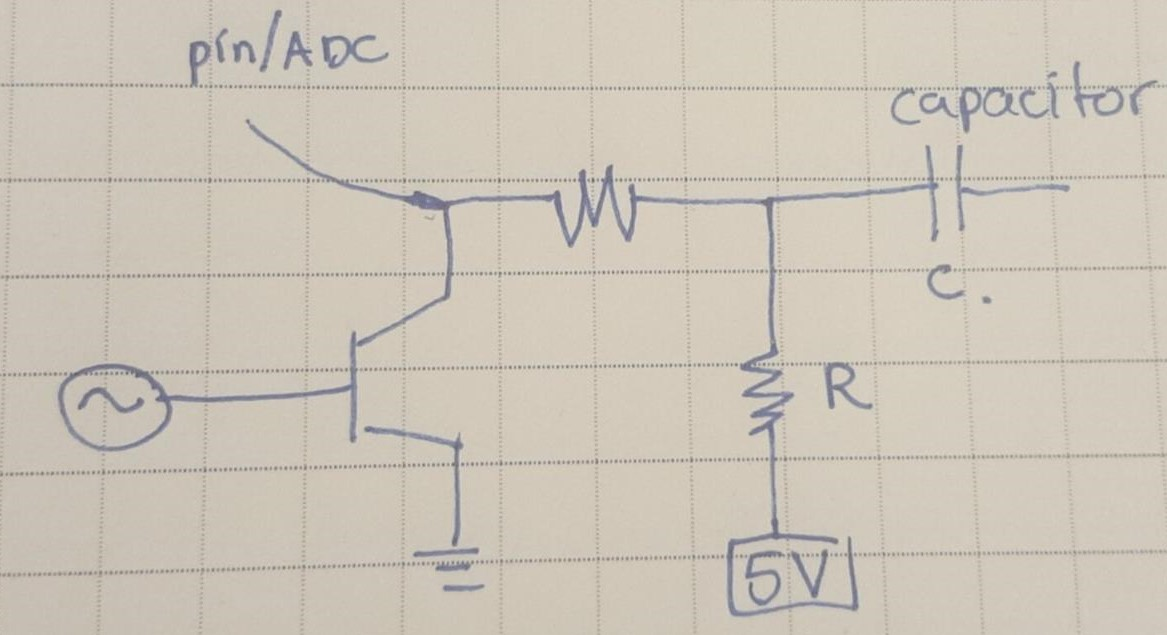
\includegraphics[width = 50mm]{Pics/4-24c.jpg}  \end{center}
I am able to sense when I touch the cardboard aluminum foil capacitor plate, but I am unable to get a different capacitor RC time constant reading when I vary my hand distance from the aluminum foil. 
\\ I can consider designing a \href{http://www.radio-electronics.com/info/circuits/rc_notch_filter/twin_t_notch_filter.php}{twin t notch filter} to filter out the 60Hz noise. 


%%%%%%%%%%%%%%%%%%%%%%%%%%%%%%%%%%%%%%%%%%

\section{April 25 2016}

Goals I have for today / {\bf done} if task completed
\begin{tight_itemize}
\item Finalize design for my user input % {\bf done}
\item Look into connecting PSoC to 8051 and VGA display
\item Continue Building my 3D Tic Tac Toe AI {\bf [done]}
\end{tight_itemize}

\subsection{Designing the Capacitance Based Sensor } 
This is the twin t notch filter that I have in mind: 
\begin{center} 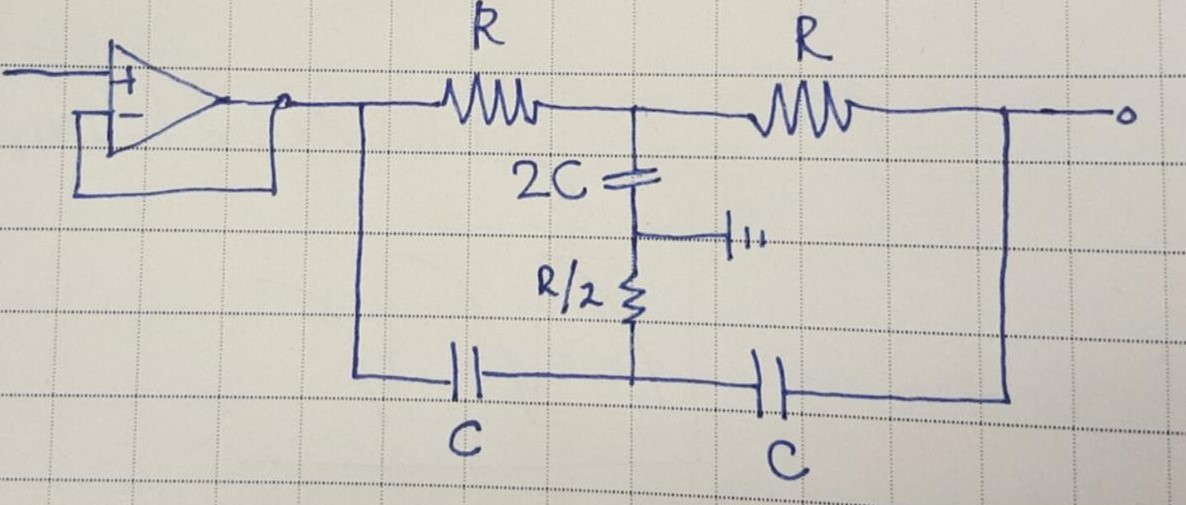
\includegraphics[width = 50mm]{Pics/4-25a.jpg}  \end{center}
The formula for the cutoff frequency is $f_c = \frac{1}{2\pi RC}$, and I am using $C = 100pF$ and $R = 27k\Omega$. However, I am unable to filter out a default 60Hz. 

\subsection{Connecting PSoC to 8051}
Check out \href{http://web.mit.edu/6.115/www/document/cable_blackbird.pdf}{this link} to see how to connect my 8051 to my PSoC. 
\\ Today, I soldered the Sparkfun connector piece, and I got the LA checkoff showing that I could successfully power my PSoC using R31JP power. I finished the pdf linked above and got the following to display:
\\ (insert image)

\subsection{Using the 74LS245}
The purpose of the 74LS245 chip is to connect my PSoC to a VGA display, so I can effectively visualize the 3D tic tac toe game. 

\subsection{Building my 3D Tic Tac Toe AI}
\begin{wrapfigure}{R}{0.42\textwidth}
\centering
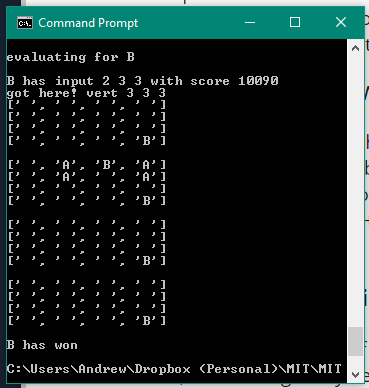
\includegraphics[width = 0.4\textwidth]{Pics/4-25b.png} 
\end{wrapfigure}
I completed building my AI for my 3D Tic Tac Toe Game in python today. I thought about running a brute force tree search to exhaust all combinations of the 3D Tic Tac Toe Game, but that would be on the order of 64! moves and would be a bit complicated. Instead, I wrote an evaluation metric to evaluate the values of certain locations on the boards, and the AI would place its next move based on the highest scoring location. My scoring works as follows, for a certain row/diagonal of 4 that does not have both an AI and player move:
\begin{tight_enumerate}
\item If the AI has a 3 in a row, connect it
\item If the opponent has a 3 in a row, block it
\item If the opponent has a 2 in a row, block it
\item If the AI has a 2 in a row, connect it
\item If the AI has a 1 in a row, connect it
\item If the row has nothing, add a move
\item If the opponent has a 1 in a row, block it
\end{tight_enumerate}
The cumulative sum of the scores after checking all potential connect 4 paths will determine the next place to play. You can take a look at the code \href{https://github.com/qandrew/6.115-final-project/blob/master/Code/tic_tac_toe_ai.py}{here}.
\\
\\ As for further work to be done, I should (a) port the game to C to put on the PSoC, (b) consider difficulty settings for the game, (c) WORK ON THE HARDWARE ASPECT!

%%%%%%%%%%%%%%%%%%%%%%%%%%%%%%%%%%%%%%%%%%

\newpage
\section{April 26 2016}

Goals I have for today / {\bf done} if task completed
\begin{tight_itemize}
\item Connect PSoC to VGA display % {\bf done}
\item Port 3D Tic Tac Toe to C {\bf done}
\item Buy capacitance based sensing chips
\end{tight_itemize}

\subsection{Connect PSoC to VGA display}
I got a PSoC module from Prof. Leeb today that will allow me to connect my PSoC to the module using a Serial Port, and the module will convert the serial port data to something displayable on the monitor display through a VGA display port. 
\\ I acquired a null modem cable and a male-to-female serial cable, which will allow me to connect my R31JP to the PSoC-based VGA board. See \href{http://web.mit.edu/6.115/www/document/psoc_vga_manual.pdf}{this document} for more help.

\subsection{Port 3D Tic Tac Toe to C}
I also spent time at home and booted into my Ubuntu and ported my python Tic Tac Toe code to C. I now have a working two player version that can run on terminal, and I plan to write the AI maybe the next day and get it running on my PSoC soon. 


%%%%%%%%%%%%%%%%%%%%%%%%%%%%%%%%%%%%%%%%%%

\section{April 27 2016}

Goals I have for today / {\bf done} if task completed
\begin{tight_itemize}
\item Connect 8051 to VGA display {\bf done}
\item Connect PSoC to VGA display {\bf done}
\item Port 3D Tic Tac Toe code to PSoC
\end{tight_itemize}

\subsection{Connect 8051 to VGA display}
Following the instructions from \href{http://web.mit.edu/6.115/www/document/psoc_vga_manual.pdf}{this document}, I wrote a simple \texttt{vga.asm} file to display red and green stripes on a VGA display. Consult the image below to see my display.
\begin{center} 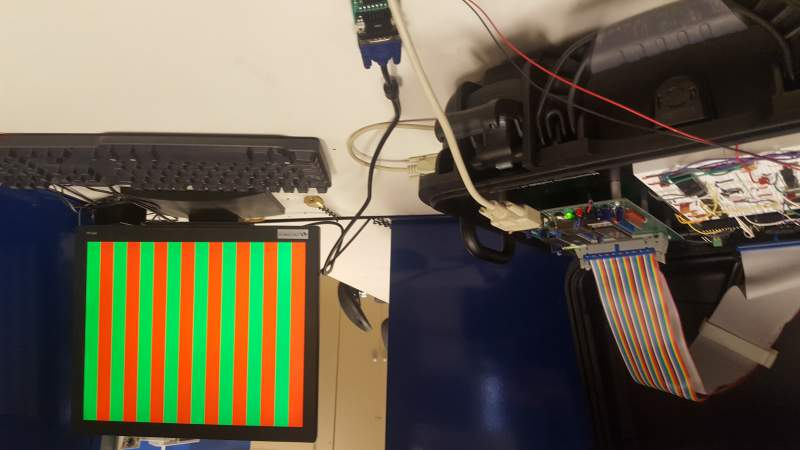
\includegraphics[width = 80mm]{Pics/4-27a.jpg}  \end{center}

\subsection{Connect PSoC to VGA display}
Using the PSoC on a board, I was also able to connect my PSoC 5 to the VGA display. I am using the \textsc{UART\_PutChar()} function to write to serial. I am also powering the 5V PSoC on a board using a phone charger that I took apart. 
\\
\\ Eventually, I will construct a simple circuit to connect my PSoC to my VGA display board using a 74LS245 chip. The 74LS245 datasheet can be found \href{../Datasheets/74LS245.pdf}{here} or \href{http://www.futurlec.com/74LS/74LS245.shtml}{here}. Below is a schematic of the desired circuit:
\begin{center} 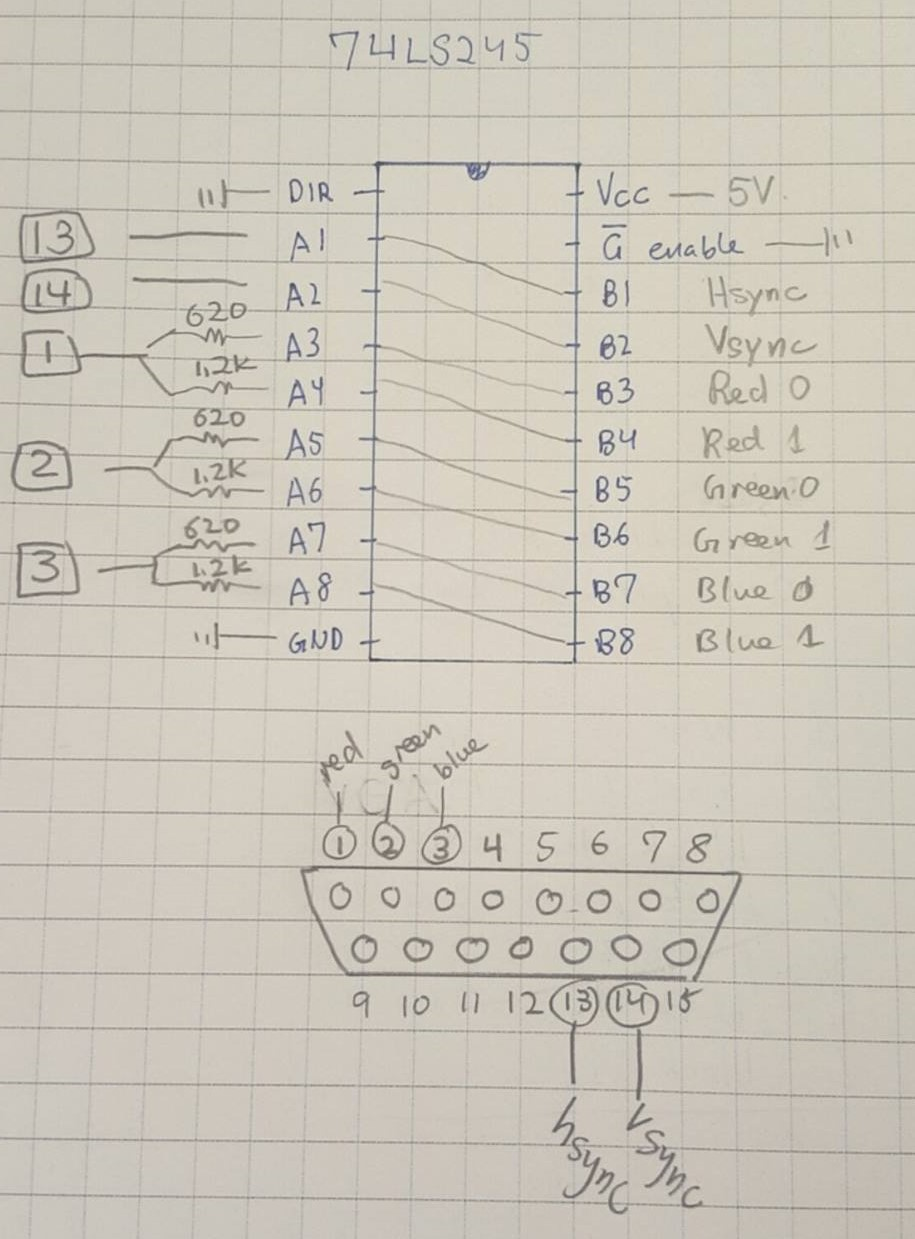
\includegraphics[width = 80mm]{Pics/4-27b.jpg}  \end{center}
I will first try to get my game running using the PSoC on a board before creating my own wiring schematic.

%%%%%%%%%%%%%%%%%%%%%%%%%%%%%%%%%%%%%%%%%%

\newpage
\section{April 28 2016}

Goals I have for today / {\bf done} if task completed
\begin{tight_itemize}
\item Display Tic Tac Toe Board on PSoC {\bf done}
\item Port Tic Tac Toe Code to PSoC {\bf done}
\end{tight_itemize}

\subsection{Display Tic Tac Toe Board on PSoC}
I am running some problems while trying to program my PSoC. I have been getting \texttt{Build error: The command 'arm-none-eabi-gcc.exe' failed with exit code '1'.} multiple times, even when I remodify the code to the original state the message does not dissappear. I will need to debug this.
\\ Apparently the solution to this is to not \texttt{\#include<disp.c>} or whatever file that I need to include; it seems as if the files are included implicitly. However, I need to declare structures in the \texttt{main.c} file; see my April $29^{\text{th}}$ \texttt{tic tac toe board displays on VGA} commit to see where my code is. I'll ask a TA and see what's up. 

\subsection{Port Tic Tac Toe Code to PSoC}
Having written my c files, ion which I can play 3D tic tac toe on my linux terminal, I will now try to run my code on the PSoC. I managed to port the two player code over, although I seem to be having some trouble with the \texttt{\#include} dependencies of my \texttt{tic\_tac\_toe\_ai.c} file that requires \texttt{tic\_tac\_toe.c}. I was, however, able to get the Tic Tac Toe board to display on my VGA. The late night was worth it. See the images below for what I got to display after each player moved once (left) and my visual layout design (right). (The Chinese character Xia is a homonym for my last name.)
\begin{center} 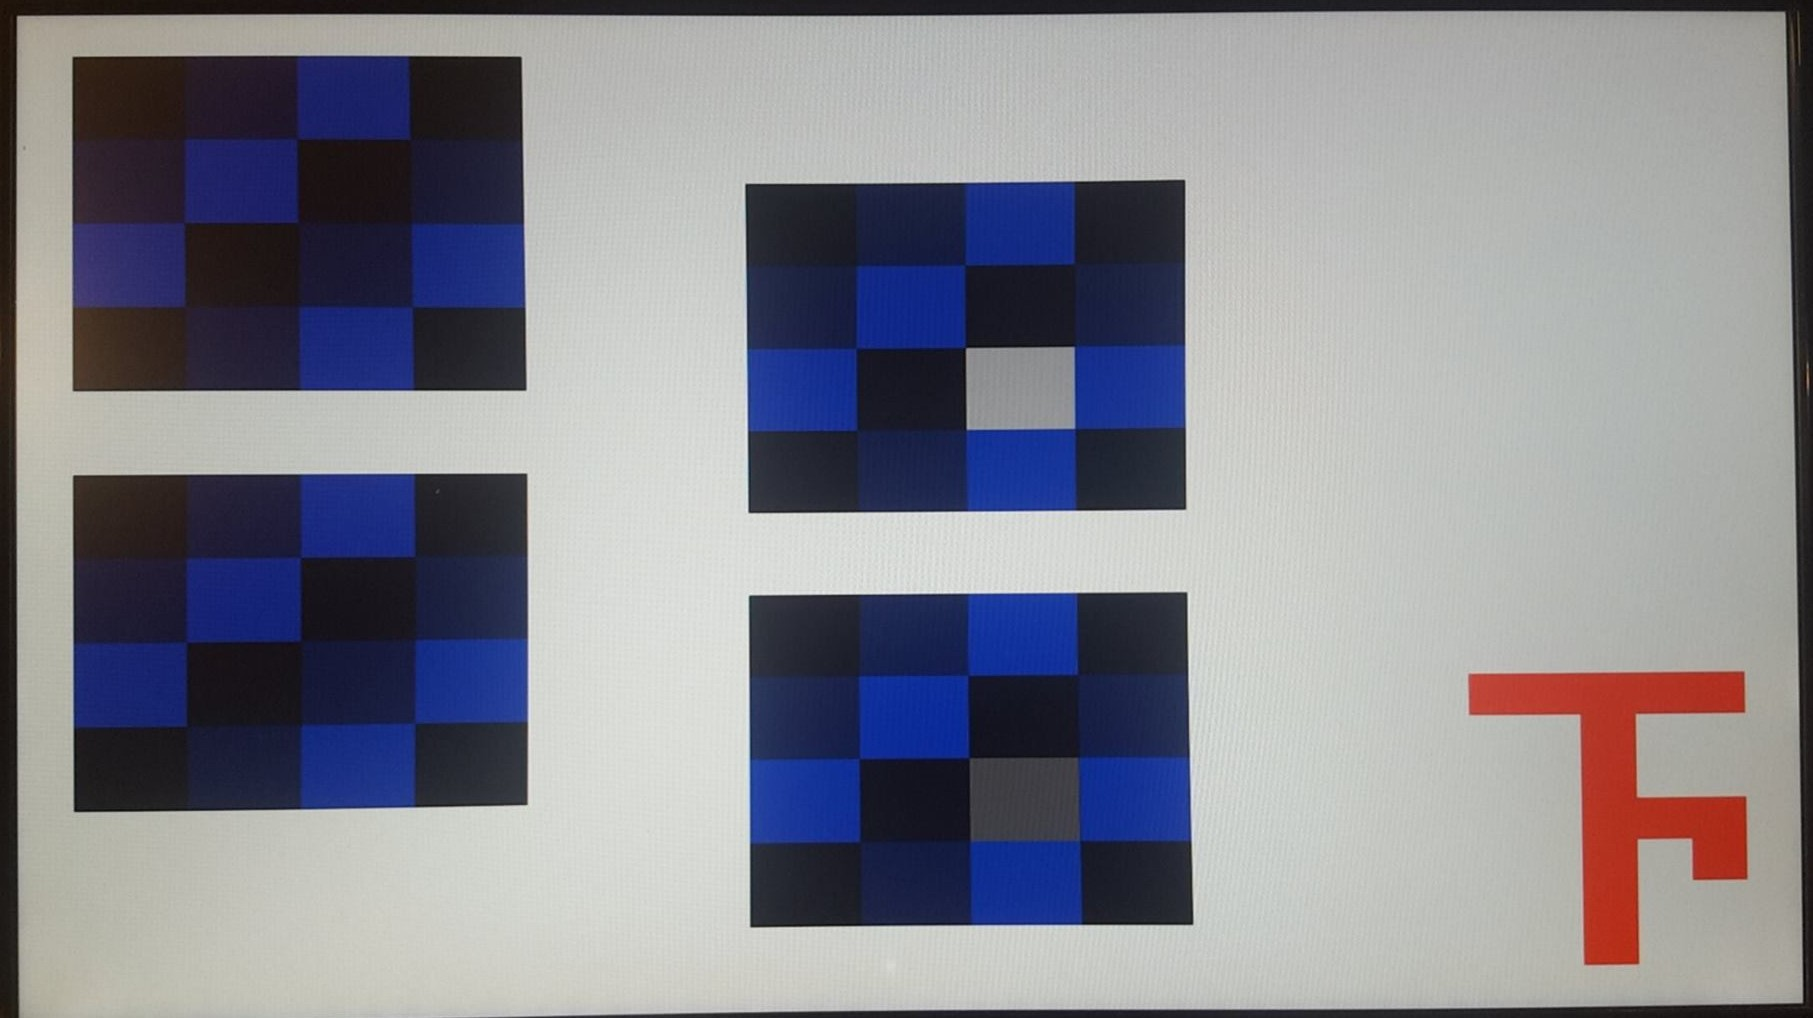
\includegraphics[width = 80mm]{Pics/4-28a.jpg}
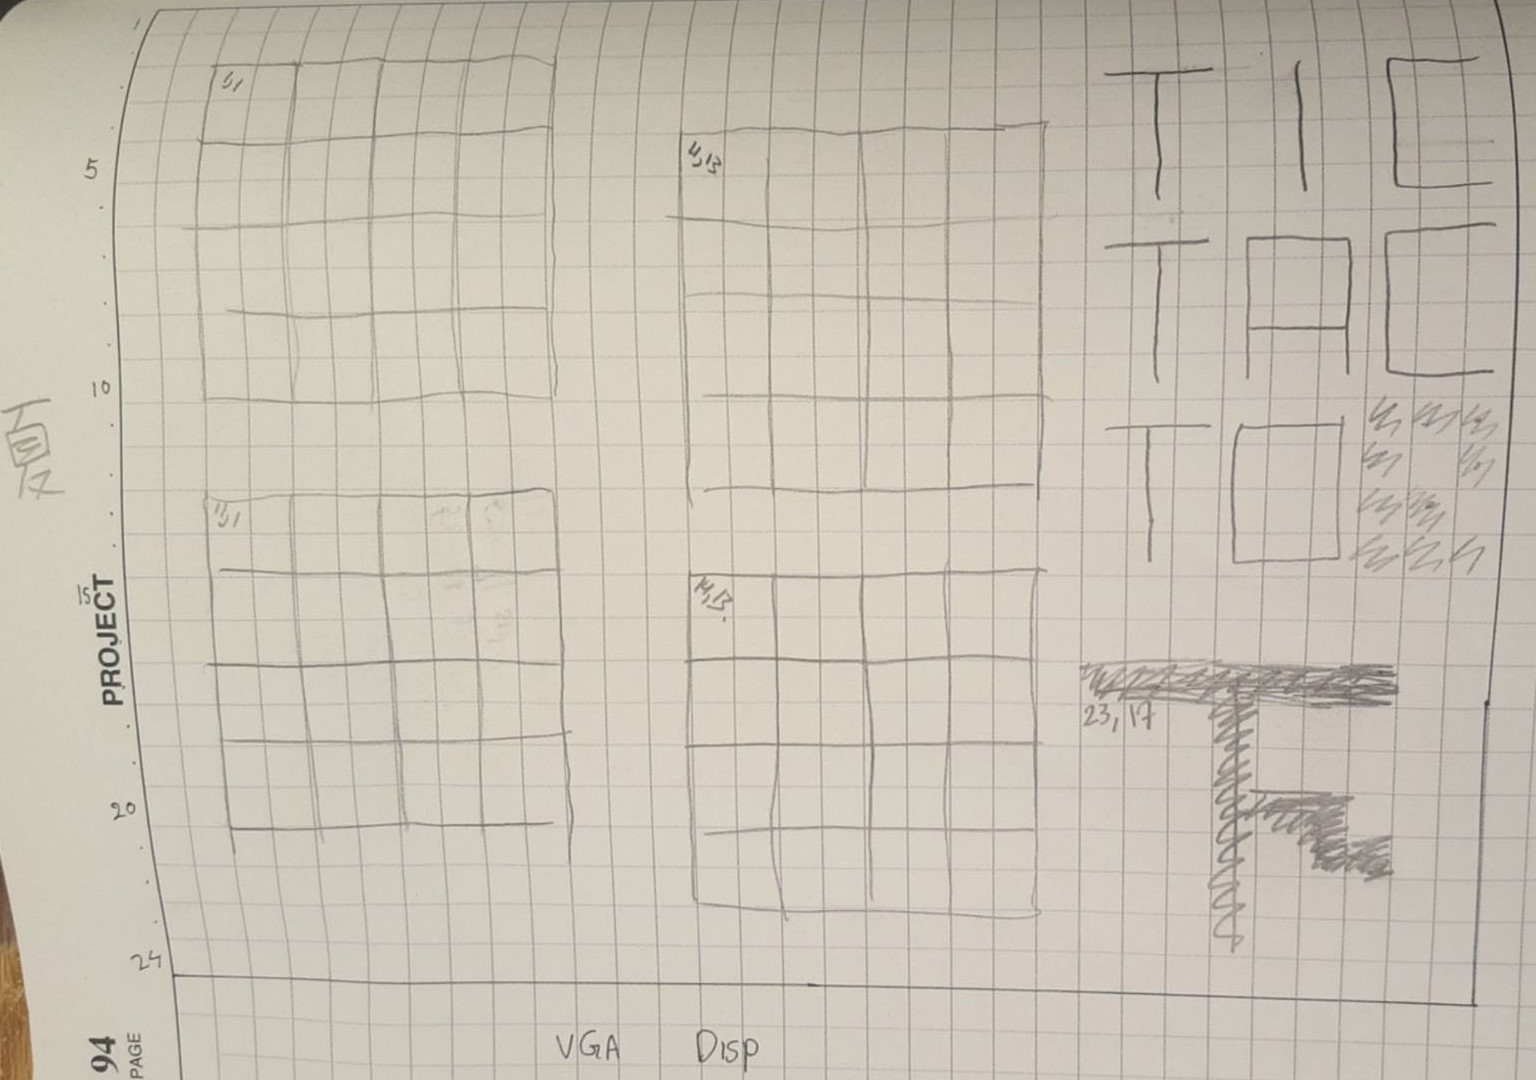
\includegraphics[width = 70mm]{Pics/4-28b.jpg}  \end{center}

Here are some further palces for improvement:
\begin{tight_itemize}
\item Learn more about C memory allocation/freeing so I do not have memory leakage
\item Think about the visual VGA display; how can I improve the aesthetics
\item Get AI working on PSoC
\item Think about my user input interface and how I want to link up the 8051
\end{tight_itemize}

%%%%%%%%%%%%%%%%%%%%%%%%%%%%%%%%%%%%%%%%%%

\newpage
\section{April 29 2016}

Goals I have for today / {\bf done} if task completed
\begin{tight_itemize}
\item Connect 8051 to PSoC via Databus {\bf done}
\item Get AI working on PSoC
\end{tight_itemize}

\subsection{Connect 8051 to PSoC via Databus}
Today, I want to connect my 8051 to PSoC via databus. First, I configured my PSoC jumpers to take 5V instead of 3.3V. 
\\ I will use port a of my 8255 on the microcontroller to send databits to Port 3 of the PSoC. I configured my port 3 to be input and {\em high impedance digital} with a low drive. You can see my code at \texttt{main.c} at my current commit \texttt{connected 8051 to PSoC via 8255 databus} to see the code I wrote. 
\\ Keep in mind that the PSoC has to be at the same ground as the microcontroller, otherwise I may get wacky 16v readings. Also, for some reason the PSoC can't read an input of 0, but I will try to fix that.  Below is an image of my PSoC LCD displaying the digital value fed from the 8255 port A. (Which I can generate by writing \texttt{WFE33 = 80; WFE30 = FD;}). 
\begin{center}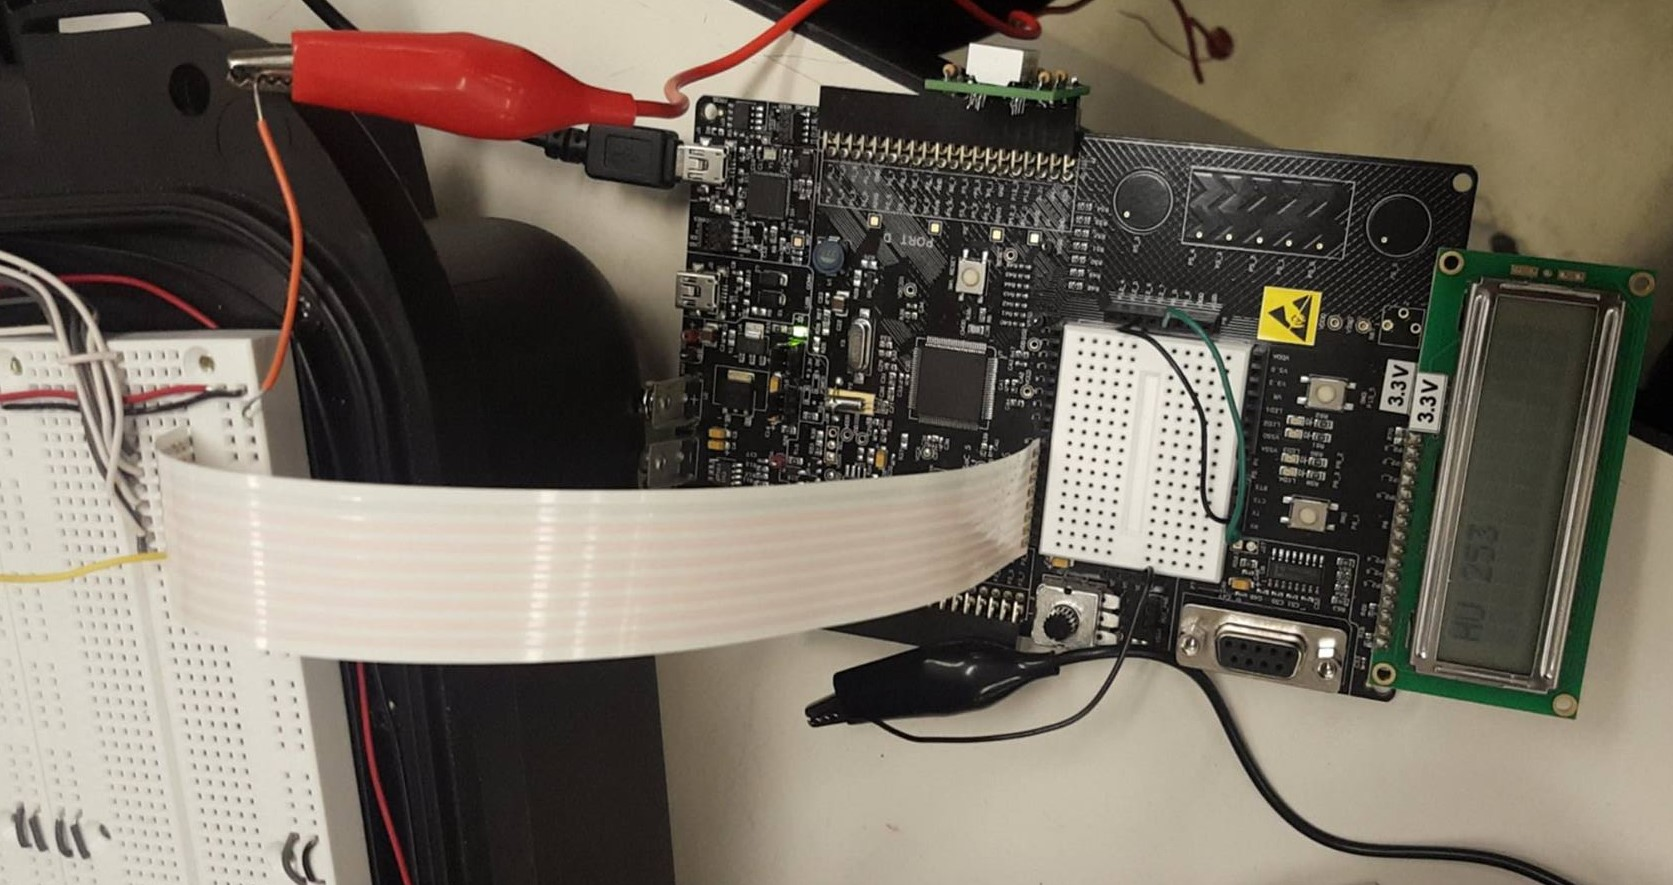
\includegraphics[width = 100mm]{Pics/4-29a.jpg}  \end{center}

\subsection{Writing software to connect 8051 to PSoC via Databus}
Now that I have the basic connection completed, I should also develop a protocol of how I want to write my code on the 8051 and PSoC side to determine when the PSoC should be reading a signal from the 8051 and when it should not be reading. (For example, if the 8255 is set at \texttt{80} all the time, I should not continuously print \texttt{80}.)
\\ I wrote \texttt{keypad\_to\_8255.asm} so now when I press a keypad, I can send the corresponding ascii value to the 8255 (and to the PSoC). However, my 8255 seems broken in the sense that PA0 is always high. I might get a new 8255. 

%%%%%%%%%%%%%%%%%%%%%%%%%%%%%%%%%%%%%%%%%%
%TEMPLATE%

\newpage
\section{May 4 2016}

Goals I have for today / {\bf done} if task completed
\begin{tight_itemize}
\item Program 8051 to be able to send Tic Tac Toe game signals to PSoC {\bf done}
\item Get AI working on PSoC {\bf done}
\end{tight_itemize}

\subsection{Program 8051 to be able to send Tic Tac Toe game signals to PSoC}
For some reason, my 8255 is not completely reliable (or maybe my PSoC port 3 isn't completely reliable). Sometimes, PA0 is unresponsively high (which means that I am only able to generate even numbers) or sometimes PA6 is unresponsively high (which pushes all ASCII values up by 64). It could also be a software 
\\ 
\\ With that said, here is a general overview of my program flow. In my 8051 code, when I press a keypad button, the 8255 sets PA the corresponding ascii symbol for $80\times256\times2$ machine cycles (this value can change; see \texttt{keypad\_to\_8255\_1.asm}, and then resets the value to 0. 
\\ The PSoC reads the values from the 8255 continuously; displaying the current read (which most of the time is 0) and the most recent nonzero read. When we get an integer input; we think of it as that the user has inputted a value, and we `play' a move on the 3D tic tac toe board. See the github commit \href{https://github.com/qandrew/6.115-final-project/commit/6c326fa8a2db2a654800f6be3b9bfd5749913904}{\texttt{can play 2d tic tac toe on vga via 8051 keypad}}. Below is a picture of the game so far: 
\begin{center}
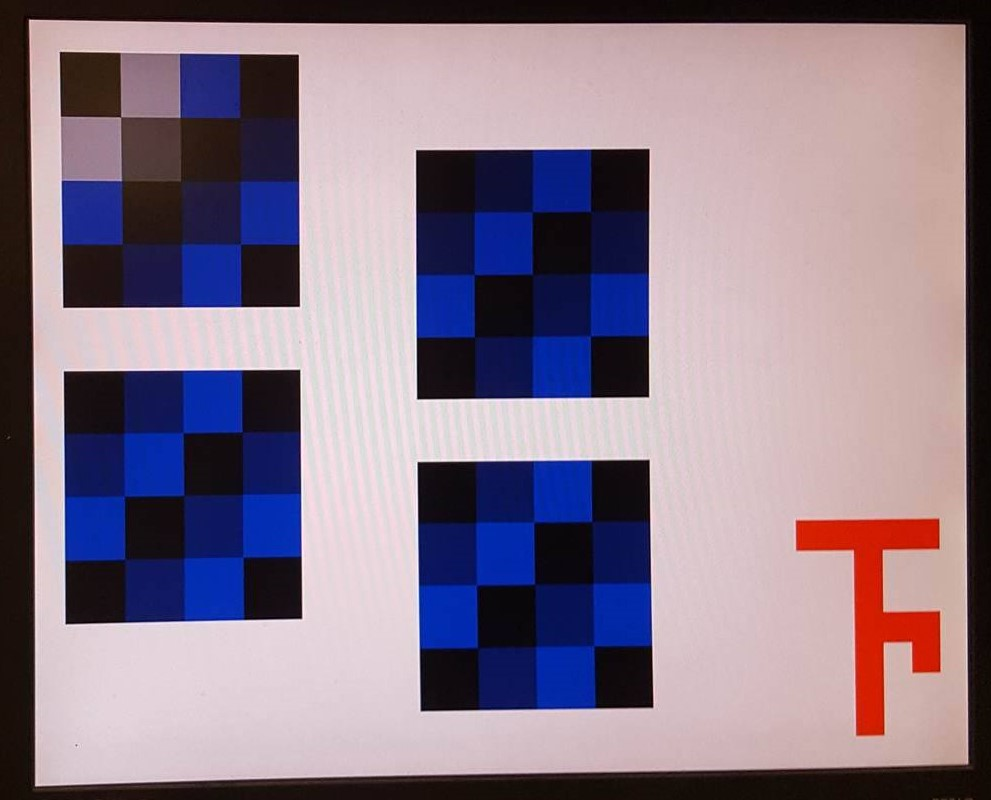
\includegraphics[width = 80mm]{Pics/5-4b.jpg}
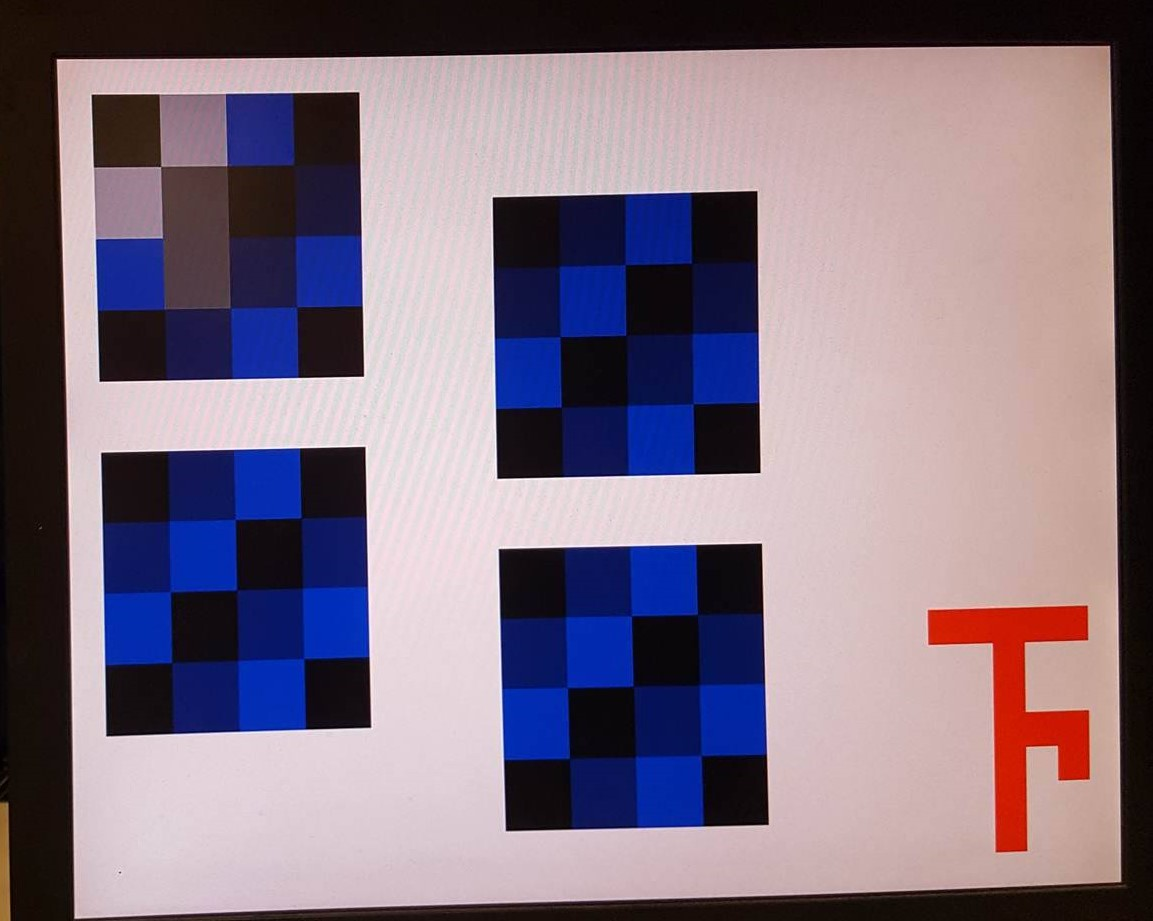
\includegraphics[width = 81mm]{Pics/5-4a.jpg}
\\ The light gray colors were fed in from the keyboard as player 1; the dark gray as player 2. From the left image to the right image, the player has placed a value at 1,2,0 \end{center}

\subsection{Get AI working on PSoC }
I'm still not exactly understanding how the implicit include in PSoC creator works, but one solution to solve this problem is to keep my AI and non-AI code in the same c file. See my \texttt{got ai to work in tic\_tac\_all.c without keypad} commit to see this stage of the project. 
\\ The solution is to include the header \texttt{disp.h} file in \texttt{main.c} in which \texttt{disp.h} defines all of the methods (and includes the structures) but does not include the c file. In fact, never include the c file.  See my \texttt{added .h files so now psoc include works} commit to see this stage of the project. 
\\
\\ The next thing I need to do is get a random seed for my random number generator (otherwise I will be generating the same random numbers every time and thus the program will no longer be random). 
\\ \indent I'll let P6\_6 be my input which will be very noisy. EDIT: not exactly working because I think as I've grounded my PSoC to the 8051 and the input noise is too predictable.
\\ \indent I'll now try to use the PSoC clock module to generate random seed bits. I will use the 8254 on my 8051 to generate random signals. 

\subsection{Two Player Game Interface Running}
I also implemented the full game tonight, that is playable using the keypad and two high/low wires into P0\_0 and P0\_1 (which are the orange wires below). Now I can input across planes. 
\begin{center}
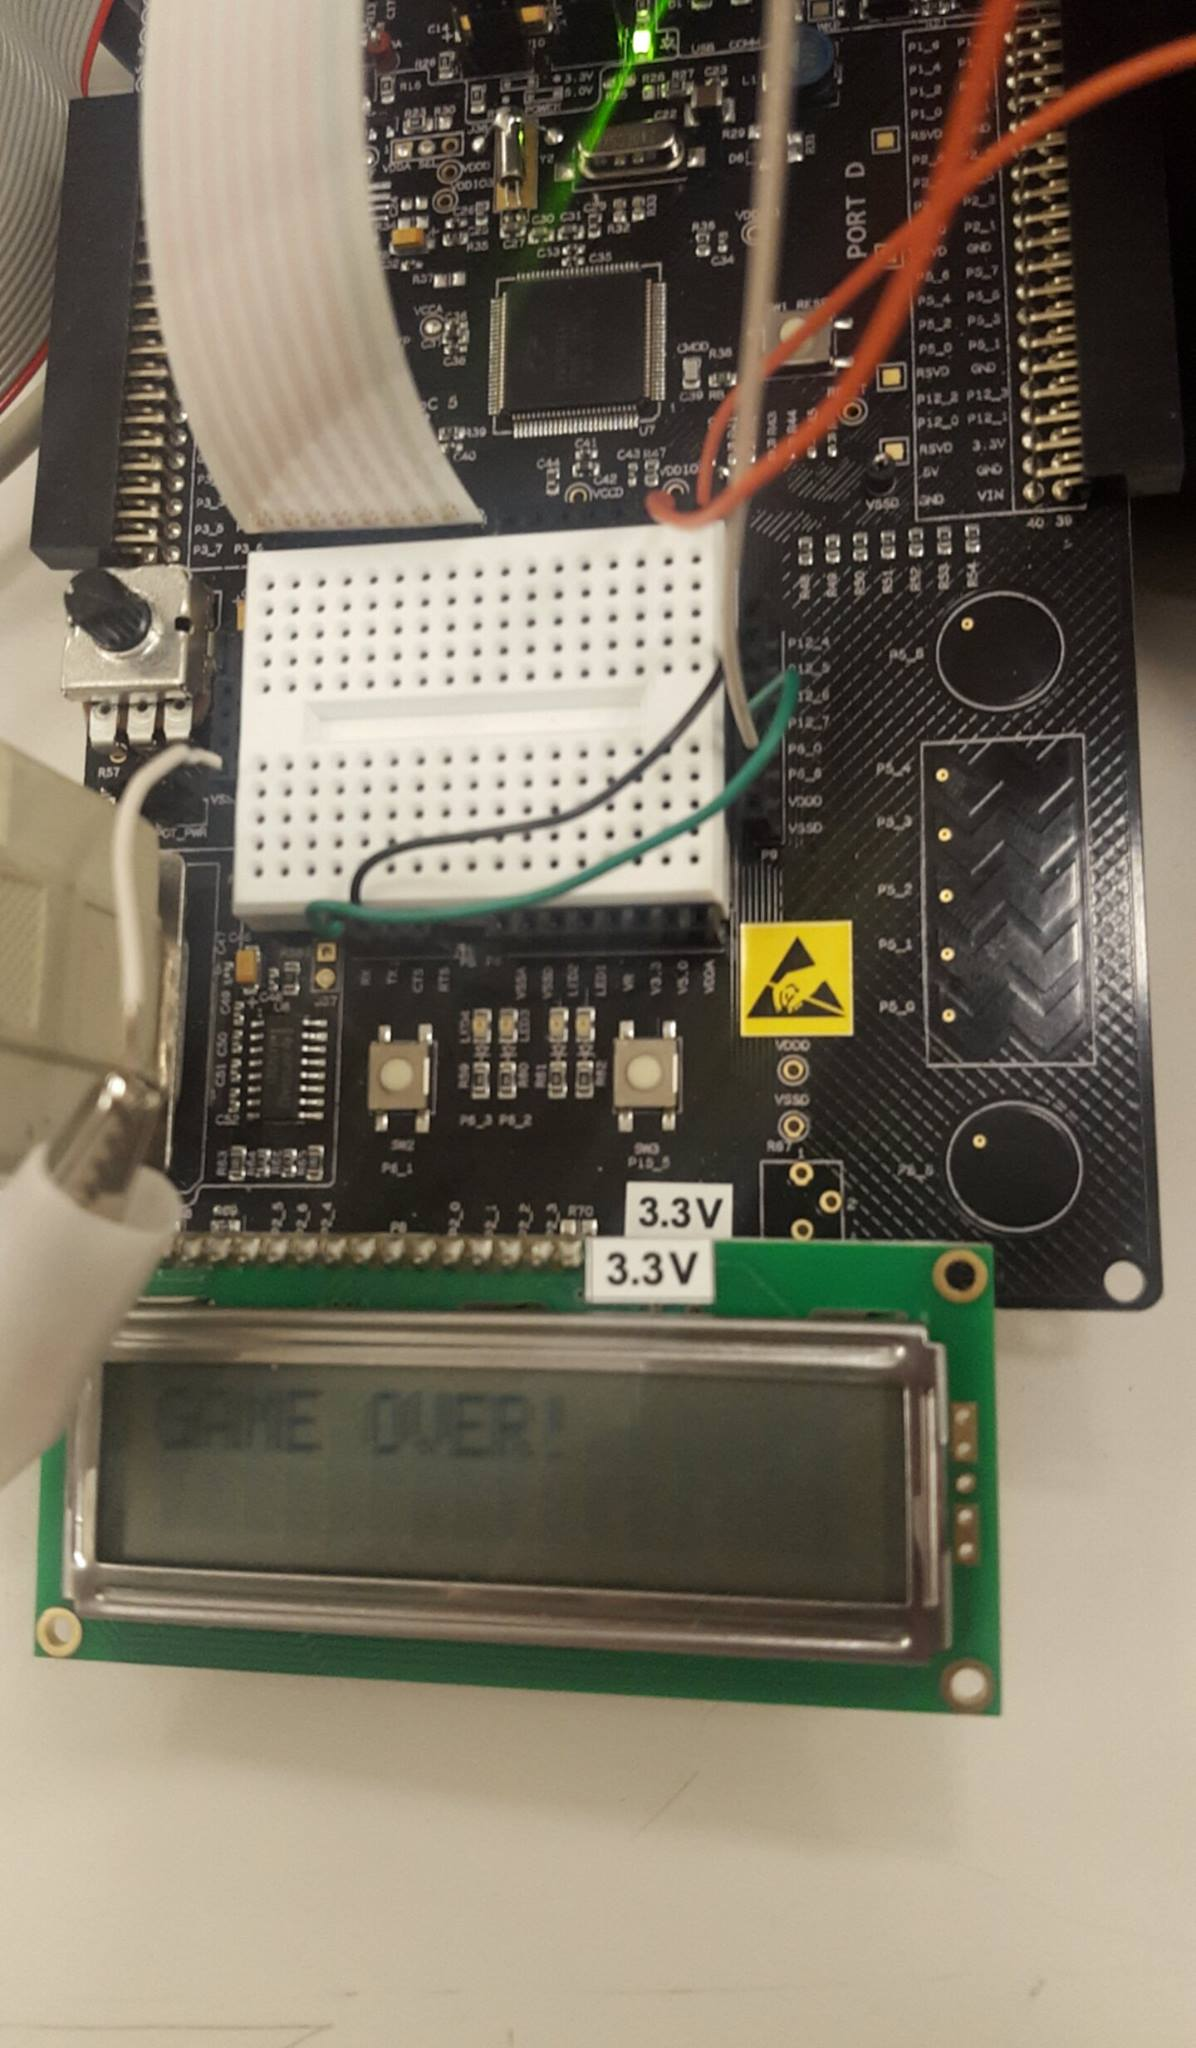
\includegraphics[width = 40mm]{Pics/5-4c.jpg}
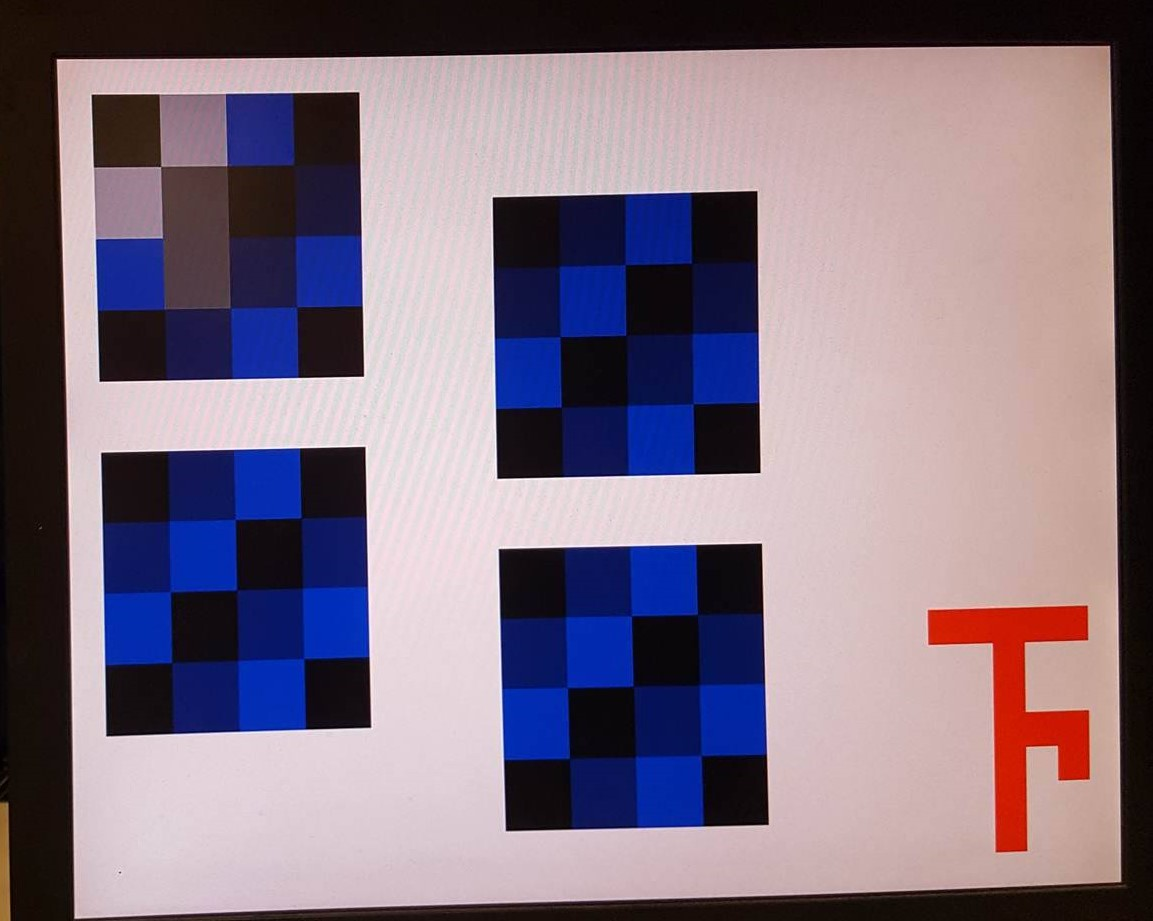
\includegraphics[width = 81mm]{Pics/5-4a.jpg}
\end{center}
I've committed the code in \texttt{random using 8254 timer, got 2 player implemented with p0 low/high cables}. 
\\ Next, I need to figure out a better user input interface. 

%%%%%%%%%%%%%%%%%%%%%%%%%%%%%%%%%%%%%%%%%%

\newpage
\section{May 6 2016}

Goals I have for today / {\bf done} if task completed
\begin{tight_itemize}
\item Get my Capacitance based sensor configured on the 8051 {\bf done}
\item Work on UI side for the PSOC 
\end{tight_itemize}

Problems I still have:
\begin{tight_itemize}
\item 8255 is unreliable
\item Do I want to configure 16c450 to communicate with the 12 pin cap sensor?
\end{tight_itemize}

\subsection{Configuring the capacitance based sensor}
I bought capacitance based sensors from \href{https://learn.adafruit.com/adafruit-capacitive-touch-sensor-breakouts/overview}{Adafruit}. The datasheets are also located through that link. The 12 pin datasheet can be found \href{https://www.sparkfun.com/products/9695}{here}. The chips look like this:
\begin{center}
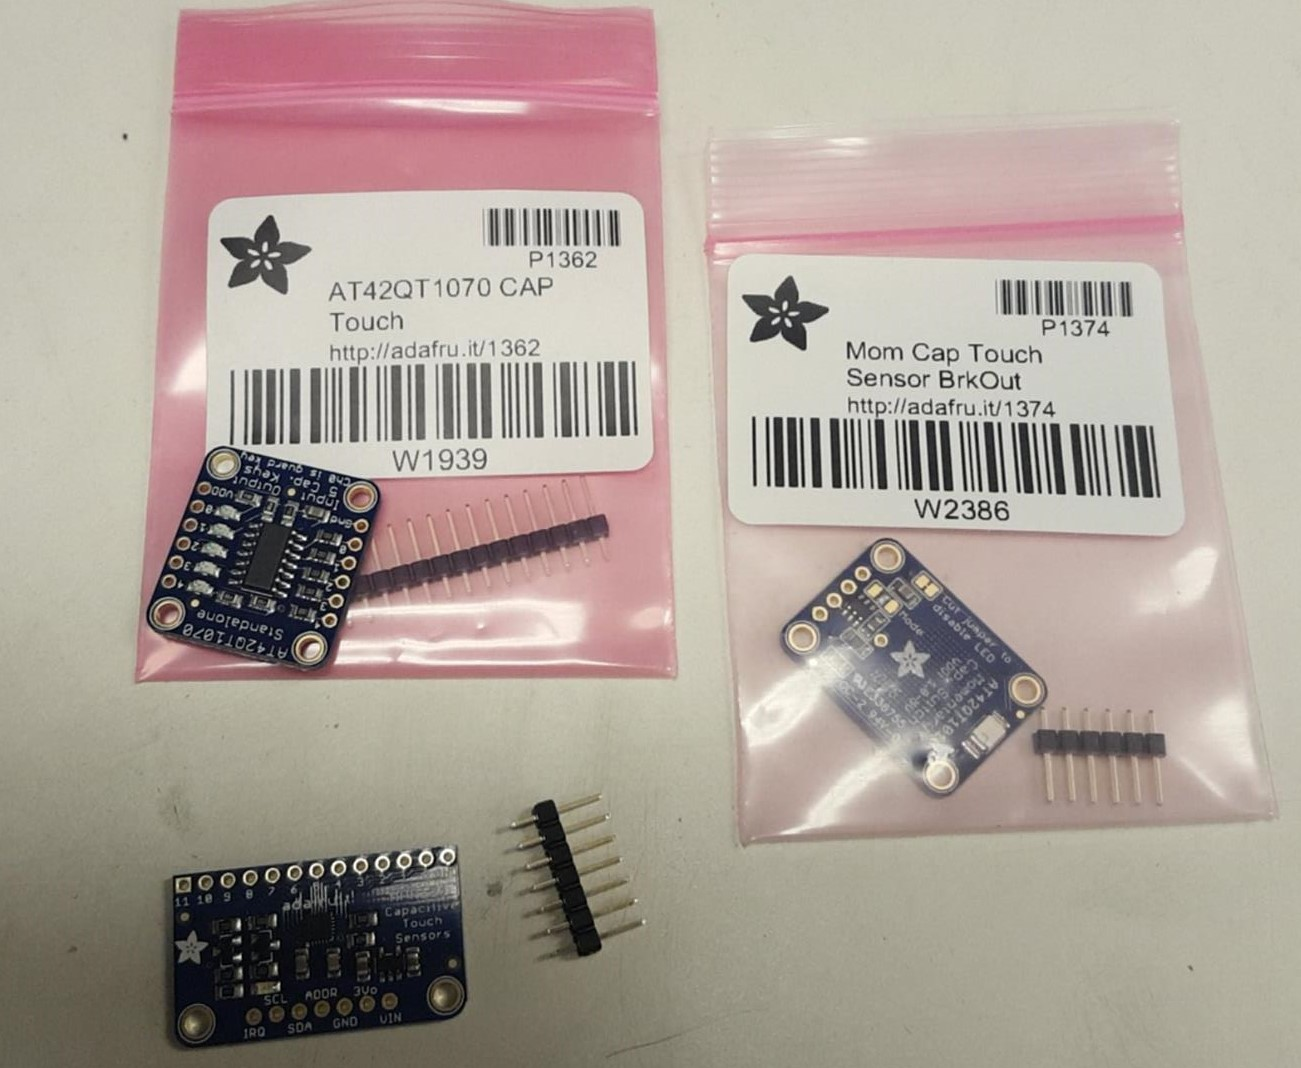
\includegraphics[width = 80mm]{Pics/5-6a.jpg}
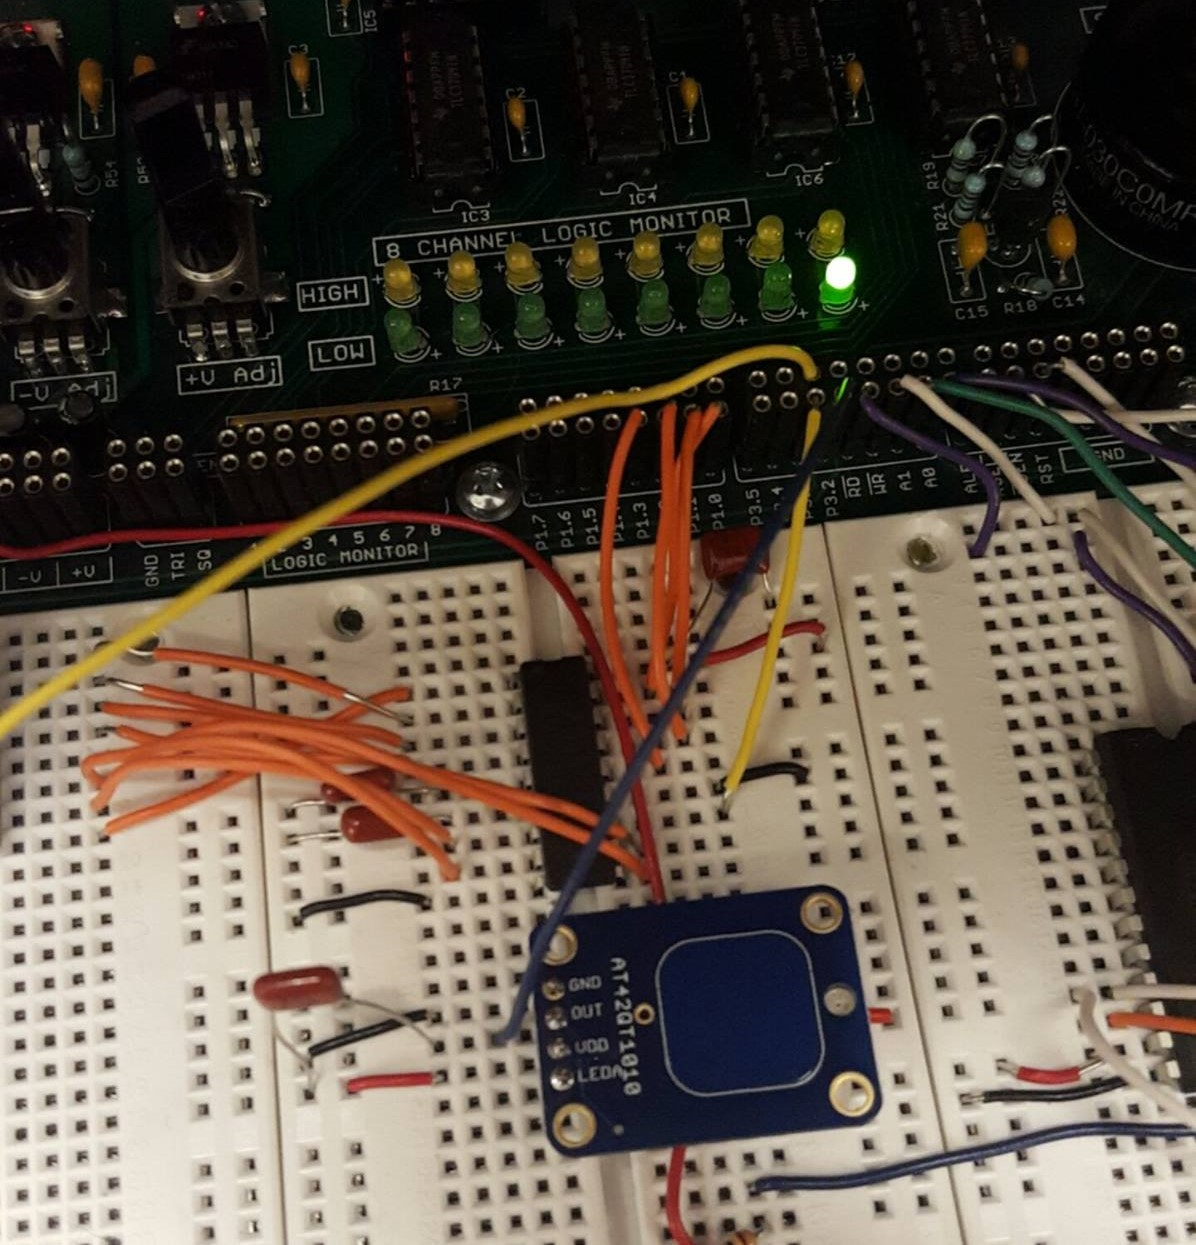
\includegraphics[width = 63mm]{Pics/5-6b.jpg}
\end{center}
The picture in the left are the three chips I bought. The picture on the left is my connected 1010 cap sensor (touch the blue square area to activate) in an interrupt configuration. 
\\ For now, I am writing a script so I can detect when I have pressed on the 1010 cap by using interrupts. \href{http://www.circuitstoday.com/external-interrupts-handling-in-8051}{This} is a nice reference link. I have written the interrupt code in \texttt{keypad\_with\_cap.asm}; please refer to commit \texttt{added capacitave chip interrupt code}. I have 
\\
\\ Side note: The 12 pin MPR121 seems to require serial communication; so I'll have to configure my 16c450 chip. 

%%%%%%%%%%%%%%%%%%%%%%%%%%%%%%%%%%%%%%%%%%
%TEMPLATE%

\newpage
\section{DATE 2016}

Goals I have for today / {\bf done} if task completed
\begin{tight_itemize}
\item Task % {\bf done}
\item Task 
\end{tight_itemize}

\end{document}